\chapter{実装}
\label{implementation}

\ref{kadai}節を踏まえつつ\ref{proposed}節で解決に近づけるために、本章では3つの実験とその設定内容について述べる。

本章では本研究における実装環境,提案手法の実装,提案手法の評価に用いるデータセットについて述べる.
実装環境 (\ref{impl_env})では本研究における実験のための実行環境及び事前知識について述べる。
\ref{exp_common}では、K-AFの性能を最も引き出す可能性がある、学習の設定を調査する。
実験1 (\ref{exp1})ではK-AFの性能を既存の活性化関数と比較する実験を行う。また、関数の形状を学習すると同時にどのように損失関数が小さくなるかValidationLossのグラフを取得する。
実験2 (\ref{exp2})では各データセットにおいての活性化関数の形を調査する実験を行う。
実験3 (\ref{exp3})では、K-AFの性能を最も引き出す可能性がある、学習の設定を調査する。

これら3つの実験を踏まえて、K-AFの課題に対しての実用性だけでなく、K-AFの性質についても調査し、今後の発展のための鍵となる結論へとつなげる。



\section{実装環境}
\label{impl_env}



本研究において利用した実装環境を \ref{impl_table} に示す. 提案手法の実装は Pytorch 及
を用いた.  PyTorch~\cite{pytorch}, Chainer~\cite{chainer},  Tensorflow~\cite{tensorflow} は計算グラフの自動微分ライブラリであり, 深層ニューラルネットワークの研究や開発にも用いられる.
Pytorchを用いた理由は実装コストが低く研究領域に従事できるところにある。


\begin{table}[htbp]
    \begin{center}
        \caption{本研究の実行環境}
        \label{impl_table}
        \vspace{2mm} 
        \begin{tabular}{|c|c|}
        \hline
        環境              & バージョン \\
        \hline
        CPU               & Intel core i7 6コア 2.2GHz \\
        \hline
        メモリ             & 16GB \\
        \hline
        Python            & 3.8.5  \\
        \hline
        scikit-learn      & 0.23.2\\
        \hline
        numpy             & 1.18.5 \\
        \hline
        pytorch           & 2.5.0 \\
        \hline
        \end{tabular}
    \end{center}
\end{table}



\section{本実験での共通項目}
\label{exp_common}

実験に用いる活性化関数の形を図\ref{k-af-net}に示す。
\begin{figure}[hbtp]
    \begin{center}
        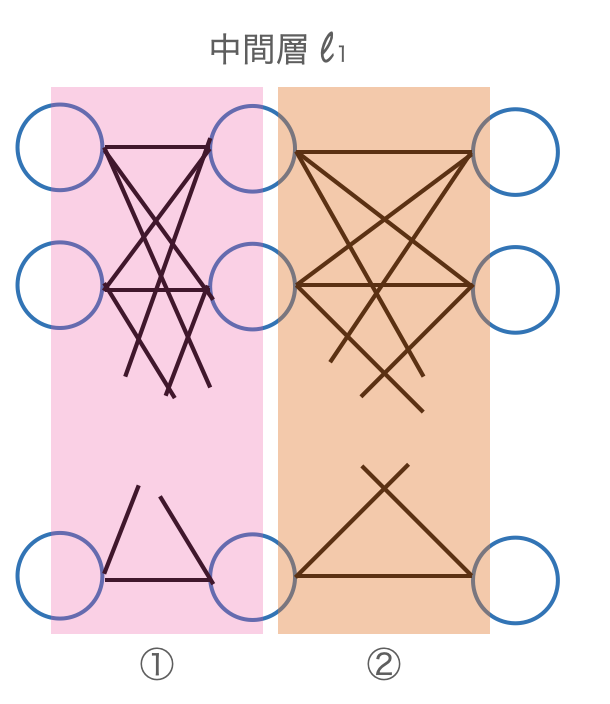
\includegraphics[width=10cm]{asset/k-af-net.png}
            \caption{実験で用いるニューラルネットワークの概要図}
            \label{k-af-net}
    \end{center}
\end{figure}

今回の実験では、簡易的なモデルで活性化関数の性能を試していく。
中間層の数を$ l_1 $とし、\textcircled{\scriptsize 1}にはReLUを用いる。\textcircled{\scriptsize 2}の部分を可変的にさまざまな活性化関数へと変えていく。
本論文で提案する、K-AFは\textcircled{\scriptsize 2}の部分において性能を評価する。

比較用の活性化関数には以下の表\ref{list:af_table}に記述してあるものを用いる。


\begin{table}[htbp]
    \begin{center}
        \caption{本実験で使用する活性化関数リスト}
        \label{list:af_table}
        \vspace{2mm} 
        \begin{tabular}{ |c| }
        \hline
        ReLU \\
        Sigmoid \\
        Tanh   \\
        Mish  \\
        Swish  \\
        K-AF(本手法)   \\
        \hline
        \end{tabular}
    \end{center}
\end{table}



活性化関数の性能の比較実験のために、以下の表項目\ref{list:learning_algorithm_change}を変えながら実験する。
データセットにはsckit-learn~\cite{scikit-learn}のライブラリのデータセットに対してデフォルトで入ってるものを想定する。
各種データセットの詳細については\url{https://scikit-learn.org/stable/datasets/toy_dataset.html}こちらのページが参考になる。



\begin{table}[htbp]
    \begin{center}
        \caption{学習においての使用するニューラルネットワークの学習アルゴリズム}
        \label{list:learning_algorithm_change}
        \vspace{2mm} 
        \begin{tabular}{ |c|c| }
        学習においての変更項目 & 変更のリスト\\
        \hline
        LearningRate           & [  $10^{-1}$,  $10^{-2}$,  $10^{-3}$,  $10^{-4}$, $10^{-5}$, $10^{-6}$ ,$10^{-7}$]    \\
        Initializer         & [ Xavier, KaimingUniform]   \\
        Regularizer           & [ 何もなし, L1ノルム, L2ノルム]     \\
        Optimizer         & [ SGD, Momentum, AdaGrad, Adam]   \\
        データセット &  [ iris, digits, wine, boston, breast\_cancer ]    \\
        \end{tabular}
    \end{center}
\end{table}



\subsection{比較データ}

他の活性化関数と適当に比較するために、以下の条件を比較して実験を行う。


\begin{table}[htbp]
    \begin{center}
        \caption{実験に用いるデータセットの情報}
        \label{dataset_name}
        \vspace{2mm} 
        \begin{tabular}{ |c|c|c|c|c|c| }
        データセット名 & サンプル数 & 入力の次元 & 出力の次元 & 出力の形式 & 中間層の数 $ {l_1} $ \\
        \hline
        iris           & 150    & 3         & 3        & 分類      & 4 \\
        digits         & 1797   & 3         & 64       & 分類      & 100 \\
        wine           & 178    & 3         & 13       & 分類      & 40 \\
        boston         & 506    & 13        & 1        & 回帰      & 20 \\
        breast\_cancer & 569    & 30        & 2        & 分類      & 30 \\
        \end{tabular}
    \end{center}
\end{table}


\subsection{実装における留意点}
実験のために必要なハイパーパラメータとして以下のパラメータを実験前に設定することとした。

\begin{table}[htbp]
    \begin{center}
        \caption{本実験において使用するハイパーパラメータ}
        \vspace{2mm} 
        \scalebox{0.7}[0.7]{
            \begin{tabular}{||c | c |c||}
            ハイパーパラメータ & 記号 & 説明 \\
            \hline
            epoch数                           & epoch\_num      & 学習の速度、最終的なValidationLossを見るのに十分なepoch数を取る。  \\
            実験回数                           & exp\_num     & 数回実験を行なった平均をとり、結果を保証する。 \\
            カーネル密度推定に用いるデータ数        & calc\_num           & $ \mathbf{X}^{calc} $ に用いるデータ数を表す。  \\
            \end{tabular}
        }
    \end{center}
\end{table}

また本論文の実験では学習の手法として、オフライン学習(バッチ学習)により全ての実験を行なった。そのためepoch数は学習の際にループで回した回数に相当する。



\section{実験1 既存の活性化関数との比較実験}
\label{exp1}
\subsection{実装手法}

表\ref{list:learning_algorithm_change}に記述した5つのデータセットを軸に\ref{list:af_table}の活性化関数での比較実験を
LearningRate、Optimizer、Initializer、Regularizerを変更しながら実験した。
K-AFの性能が有利にならないように、可能な限り任意の組み合わせで実験を行い性能の評価を行う。



\subsection{評価手法}

回帰問題と分類問題におけるれぞれの評価時における精度指標(Metrics)として、
回帰問題では平均絶対誤差(MAE)を、分類問題では正解率(Accuracy)を用いる。
これらは、最も基礎的で一般的な評価関数である。

また本実験ではValidationDataはTrainingDataと等しいものとして実験を進める。


\subsubsection{MAEの数式}


評価に用いる推論したデータの集合$n$個を$ y_i \sim_n \mathcal{D}$と正解のラベル$ y_i^{true} $

\begin{eqnarray}
\mathbf{MAE} = \frac{\sum_n \|y_i - y_i^{true}\|}{n}
\label{eq:accuracy}
\end{eqnarray}

で計算することとする。


\subsubsection{Accuracyの数式}

評価に用いる推論したデータの集合$n$個を$ y_i \sim_n \mathcal{D}$と正解のラベル$ y_i^{true} $

\begin{eqnarray}
\mathbf{Acc} = \frac{\sum_n \|y_i == y_i^{true}\|}{n}
\label{eq:accuracy}
\end{eqnarray}

ここで、$ \|y_i == y_i^{true}\| $とは$ y_i $と $ y_i^{true} $が等しければ$ 1 $、等しくなければ $ 0 $を表現する数式とする。

\subsection{各種データセットでの比較実験の詳細}

各種データセットではAccuracyによる性能の比較だけでなくValidationLossのグラフから学習速度を評価する。
また、step数が$0$に近い場合活性化関数によってはかなり大きな値が出力されてしまいグラフ全体が可視化に際に評価しにくくなるので、$100$から表示することとする。

\subsubsection{irisでの比較実験}
\label{impl:iris}

irisはアヤメの分類問題であり、統計学の分野で最も一般的に性能評価がおなわれるものである。
optimzerにSGDを用いRegularizerを特に使わない理由はirisは単純なデータセットのため、収束することを前提に考えているからである。
実験に用いる設定と環境を表\ref{exp:iris}に示した。


\begin{table}[htbp]
\label{exp:iris}
    \begin{center}
        \caption{irisでの実験と設定}
        \label{exp:iris}
        \vspace{2mm} 
        \begin{tabular}{ |c|c|c| }
        設定名 & 設定1 & 設定2 \\
        \hline
        LearningRate(lr)         & $ 10^{-1} $ & $ 10^{-2} $ \\
        Initializer       & KaimingUniform &  KaimingUniform \\
        Optimizer           & SGD & SGD \\
        Regularizer     & なし & なし \\
        epoch\_num       & 1000 &  1000 \\
        exp\_num         & 3 & 3 \\
        calc\_num        & 30 & 30 \\
        \end{tabular}
    \end{center}
\end{table}



\subsubsection{digitsでの比較実験}
\label{impl:digits}

digitsは数字の画像の分類問題であり、機械学習の分野で一般的に性能評価の対象として使用されるものである。
digitsは次元数が高いデータセットであるため、OptimizerにはAdamとSGD, レギュライザーにはL1ノルムとL2ノルムを使用した。
実験に用いる設定と環境を表\ref{exp:digits}に示した。

\begin{table}[htbp]
    \begin{center}
        \caption{digitsでの実験と設定}
        \label{exp:digits}
        \vspace{2mm} 
        \begin{tabular}{ |c|c|c| }
        設定名 & 設定1 & 設定2 \\
        \hline
        LearningRate(lr)         & $ 10^{-2} $ & $ 10^{-3} $ \\
        Initializer       & KaimingUniform &  KaimingUniform \\
        Optimizer           & SGD & SGD \\
        Regularizer     & なし & なし \\
        epoch\_num       & 2000 &  10000 \\
        exp\_num         & 3 & 3 \\
        calc\_num        & 36 & 36 \\
        \end{tabular}
    \end{center}
\end{table}



\subsubsection{wineでの比較実験}
\label{impl:wine}

wineとはワインの種類の判別を13個の入力次元の性質を用いて3つにカテゴライズするデータセットである。
主に決定木の性能評価に使われることが多い。本実験では以下のデータセットを用いて行う。
実験に用いる設定と環境を表\ref{exp:wine}に示した。


\begin{table}[htbp]
    \begin{center}
        \caption{wineでの実験と設定}
        \label{exp:wine}
        \vspace{2mm} 
        \begin{tabular}{ |c|c|c| }
        設定名 & 設定1 & 設定2 \\
        \hline
        LearningRate(lr)         & $ 10^{-3} $ & $ 10^{-4} $ \\
        Initializer       & KaimingUniform & KaimingUniform \\
        Optimizer           & SGD & Adam \\
        Regularizer     & なし & なし \\
        epoch\_num       & 3000 &  3000 \\
        exp\_num         & 3 & 3 \\
        calc\_num        & 27 & 36 \\
        \end{tabular}
    \end{center}
\end{table}


\subsubsection{bostonでの比較実験}
\label{impl:boston}

bostonはボストンの住宅価格を回帰で推定する問題である。K-AFが回帰問題に対しても有効であることを示すため、この実験を行う。
実験に用いる設定と環境を表\ref{exp:boston}に示した。

\begin{table}[htbp]
    \begin{center}
        \caption{bostonでの実験と設定}
        \label{exp:boston}
        \vspace{2mm} 
        \begin{tabular}{ |c|c|c| }
        設定名 & 設定1 & 設定2 \\
        \hline
        LearningRate(lr)         & $ 10^{-5} $ & $ 10^{-5} $ \\
        Initializer       & KaimingUniform  & Xavier \\
        Optimizer           & SGD & Adam \\
        Regularizer     & なし & なし \\
        epoch\_num       & 1000 &  1000 \\
        exp\_num         & 5 & 5 \\
        calc\_num        & 26 & 26 \\
        \end{tabular}
    \end{center}
\end{table}


\subsubsection{breast\_cancerでの比較実験}
\label{impl:breastcancer}

breast\_cancerは乳がんのデータセットである。実験に用いる設定と環境を表\ref{exp:breastcancer}に示した。

\begin{table}[htbp]
    \begin{center}
        \caption{breast\_cancerでの実験と設定}
        \label{exp:breastcancer}
        \vspace{2mm} 
        \begin{tabular}{ |c|c|c| }
        設定名 & 設定1 & 設定2 \\
        \hline
        LearningRate(lr)         & $ 10^{-3} $ & $ 10^{-3} $ \\
        Initializer       & KaimingUniform & KaimingUniform \\
        Optimizer           & SGD & SGD \\
        Regularizer     & なし & なし \\
        epoch\_num       & 1000 &  1000 \\
        exp\_num         & 5 & 5 \\
        calc\_num        & 29 & 285 \\
        \end{tabular}
    \end{center}
\end{table}


\vspace{-5mm} 

\section{実験2 K-AFの関数形状の調査及び損失関数の詳細調査}
\label{exp2}

2つ目の実験では推論した活性化関数の形を表\ref{dataset_name}に記載したデータセット観測し、既存の活性化関数との違いを定性評価を行う。
活性化関数の種類を分割すると以下のようになっている。
また、ニューラルネットワークの設定は表\ref{exp1}の設定で各データセットごとに二つずつ結果を取得する。

\begin{table}[htbp]
    \begin{center}
        \caption{活性化関数の関数的な意味}
        \label{af-class}
        \vspace{2mm} 
        \begin{tabular}{ |c|c|c| }
        単調増加関数か & 勾配が$ 0 $の点があるか & 上限値があるか   \\
        \hline
        ○ or × & ○ or × & ○ or ×  \\
        \end{tabular}
    \end{center}
\end{table}


表\ref{af-class}を軸に、K-AFの形状を分析し、既存の活性化関数と比べて何が違うか評価を行う。

またそのような活性化関数を計算するためのニューラルネットワークの設定を以下の表に示した設定で行う。
\begin{table}[htbp]
    \begin{center}
        \caption{実験に用いるデータセットの情報}
        \label{dataset_name}
        \vspace{2mm} 
        \begin{tabular}{ |c|c|c|c|c|c| }
        データセット名 & LearningRate & Optimizer & Initializer & Reguralizer \\
        \hline
        iris           & $ 10^{-1} $    & 3         & 3        & 分類      & 4 \\
        digits         & $ 10^{-1} $    & 3         & 64       & 分類      & 100 \\
        wine           & $ 10^{-2} $    & 3         & 13       & 分類      & 40 \\
        boston         & $ 10^{-5} $    & 13        & 1        & 回帰      & 20 \\
        breast\_cancer & $ 10^{-2} $    & 30        & 2        & 分類      & 30 \\
        \end{tabular}
    \end{center}
\end{table}







\section{実験3 K-AFの性能が上がる条件探査}
\label{exp3}
K-AFは実験の中で勾配爆発問題が発生することが発覚した。特にbostonやbreast\_cancerでは適当なパラメータで学習を開始すると、モデルが発散する可能性が高いことが実験の中からわかった。
breast\_cancerの場合の発散は本論文でも明らかになっている。
また、勾配の発散問題はパラメータの勾配を上限値でクリッピングすることである程度減らすことが知られている。
本実験では、二つの実験を行う。

\subsection{実験3.1 ニューラルネットワークの設定変更により精度向上の条件調査}
\label{exp3.1}
K-AFが一般的にどのようなニューラルネットワークの設定の場合に性能を出しやすいか表\ref{list:learning_algorithm_change}での設定をランダムに組み合わせて、評価する。
実験1 (\ref{exp1})ではデータセットとしてbostonを用いて性能評価を行う。


その際のニューラルネットワークの設定は表\ref{dataset_name}を軸に設定する。
他に実験において必要なパラメータを以下に設定する。


\begin{table}[hbtp]
    \begin{center}
        \caption{実験のデータセットの名称}
        \vspace{2mm} 
        \scalebox{1.0}[1.0]{
            \begin{tabular}{||c|c|c||}
            ハイパーパラメータ  & wineの場合 & bostonの場合 \\
            \hline
            epoch\_num                            & 5       & 5  \\
            exp\_num                           & 1000     & 1000 \\
            calc\_num        & 50           & 50  \\
            \end{tabular}
        }
    \end{center}
\end{table}

epoch\_numが少ない理由は発散するときは初期のタイミングで発散するからである。
1000回実験する中で勾配発散頻度の回数を記録する実験をこなう。
そして、各ニューラルネットの構成で記録しどの組み合わせが一番勾配発散の回数が少ないか調査する。
また、実験3.1ではLearningRateは小さい方が勾配発散の確率が減ることは自明なためLearningRateは$ 10^{-5} $で固定するものとする。




\subsection{実験3.2 クリッピングを用いた勾配発散の制御}
\label{exp3.2}
実験3.2では表(\ref{exp:boston})の設定1の条件に対してクリッピングを用いる場合とそうでない場合に勾配発散の回数がどのように変化するか実験をする。
また学習性能についての評価を行うため、勾配発散が発生しなかった場合のAccuracyを用いた比較を行う。
これにより、クリッピングがK-AFの学習に対してどの程度有効か議論する。
本実験では、式\ref{eq:hassan}の上限値$ M $を0.025で設定する。


%%% Local Variables:
%%% mode: japanese-latex
%%% TeX-master: "../bthesis"
%%% End:
